\section{Connectionist Neuron (Perceptron)}

\mode<presentation>{
\begin{frame}%{Where are we?}
    \tableofcontents[currentsection,hideallsubsections]
\end{frame}
}

\begin{frame}\frametitle{\secname}

A neuron is a computational unit for processing information. 

\question{What does a connectionist neuron compute?}\\

\pause
- A connectionist neuron is a type of neuron model which measures for a feature within an observation (a data point). It is a feature detector/extractor e.g. edge detector, above or below a threshold.

\end{frame}

\begin{frame}{A connectionist neuron's response to 1D data}
\notesonly{A connectionist neuron's response to 1D data:}

\slidesonly{
\only<1>{
\begin{figure}[ht]
     \centering
     \savebox{\imagebox}{
	 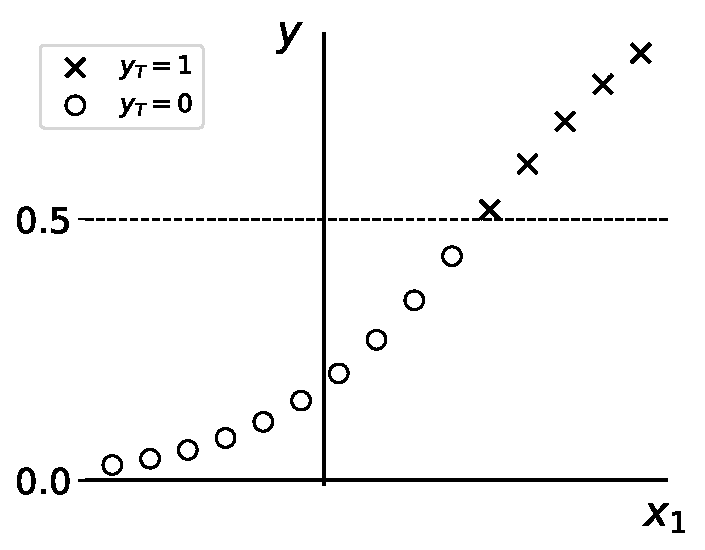
\includegraphics[width=0.3\textwidth]{img/neuron_1d_sigmoid_no-plane}}%
     \begin{subfigure}[t]{0.35\textwidth}
         \centering
         \usebox{\imagebox}% Place largest image
         \caption{}
         \label{fig:neuron_1d_sigmoid}
     \end{subfigure}
     \hspace{10mm}
     \begin{subfigure}[t]{0.35\textwidth}
         \centering
         \raisebox{\dimexpr.5\ht\imagebox-.5\height}{% Raise smaller image into place
         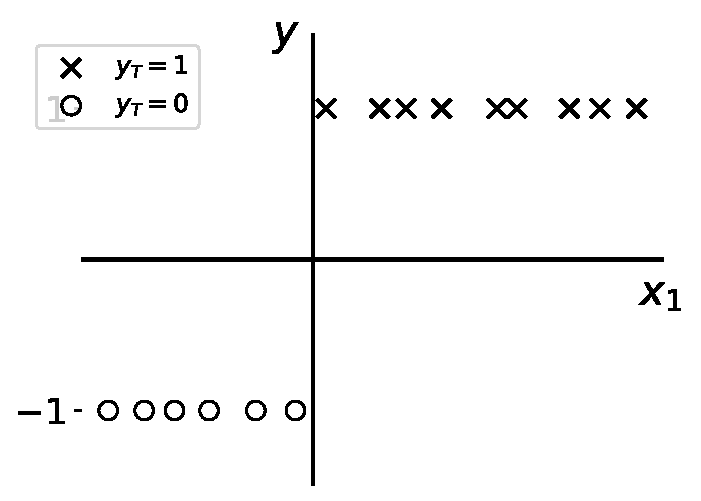
\includegraphics[width=0.9\textwidth]{img/neuron_1d_sign_no-plane}
         }
         \caption{}
         \label{fig:neuron_1d_sign}
     \end{subfigure}
     \mode<article>{
     \caption{Examples of different neuron responses to scalar input of two types: $\times$ and $\circ$. In \ref{fig:neuron_1d_sigmoid}: The neuron's response $y$ is continuous. In \ref{fig:neuron_1d_sign} the neuron repsonse is $+1$ for positive input and $-1$ otherwise. The red lines act as a decision boundary.}
	 }
	 \label{fig:neuron_1d}
\end{figure}
}
}
\only<2>{
\begin{figure}[ht]
     \centering
     \savebox{\imagebox}{
	 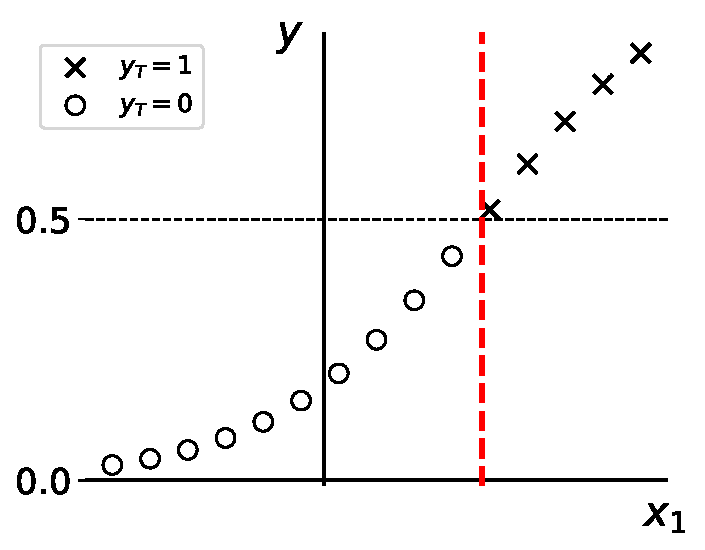
\includegraphics[width=0.3\textwidth]{img/neuron_1d_sigmoid}}%
     \begin{subfigure}[t]{0.35\textwidth}
         \centering
         \usebox{\imagebox}% Place largest image
         \caption{}
         \label{fig:neuron_1d_sigmoid}
     \end{subfigure}
     \hspace{10mm}
     \begin{subfigure}[t]{0.35\textwidth}
         \centering
         \raisebox{\dimexpr.5\ht\imagebox-.5\height}{% Raise smaller image into place
         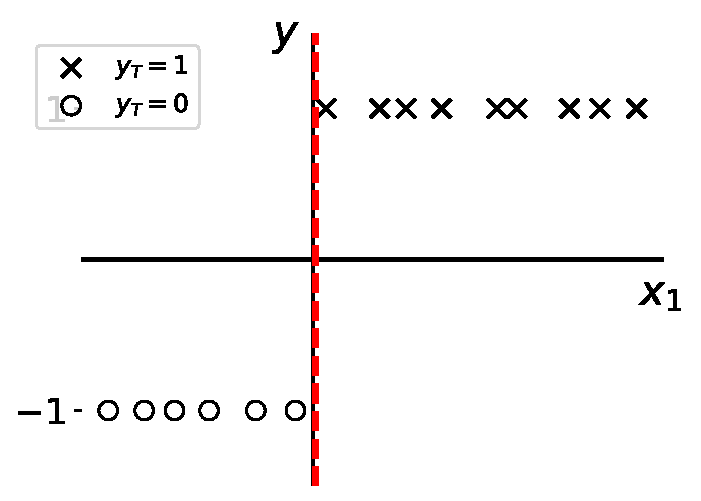
\includegraphics[width=0.9\textwidth]{img/neuron_1d_sign}
         }
         \caption{}
         \label{fig:neuron_1d_sign}
     \end{subfigure}
     \mode<article>{
     \caption{Examples of different neuron responses to scalar input of two types: $\times$ and $\circ$. In \ref{fig:neuron_1d_sigmoid}: The neuron's response $y$ is continuous. In \ref{fig:neuron_1d_sign} the neuron repsonse is $+1$ for positive input and $-1$ otherwise. The red lines act as a decision boundary.}
	 }
	 \label{fig:neuron_1d}
\end{figure}
}

\end{frame}

\begin{frame}\frametitle{
A connectionist neuron's response to 3D data:}

\begin{figure}[ht]
     \centering
     \slidesonly{
	\includegraphics<1>[width=0.4\textwidth]{img/neuron_3d_grid_no-plane}
     }
	\includegraphics<2>[width=0.4\textwidth]{img/neuron_3d_grid}
     \mode<article>{
	\caption{Examples of a neuron's response to 3D input of types $\times$ and $\circ$. Inputs of different types fall on opposite sides of a plane. The red plane acts as a decision boundary}
	}
	\label{fig:neuron_3d_grid} 
\end{figure}
\end{frame}

\subsection{Components of the connectionist neuron}
    
\begin{frame}
    
    \begin{figure}[h]
        \centering
        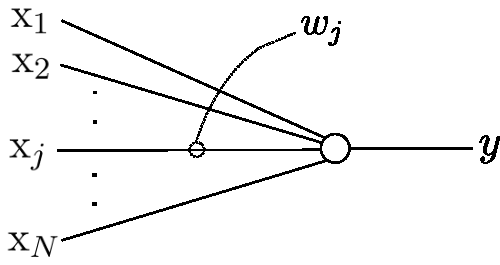
\includegraphics[height=2.3cm]{img/linearNeuron_y.pdf}
        \only<1>{
        \caption{A graphical representation of the input-output relationship for a connectionist neuron. $w_{j}$ describes the connection from the $j$-th input.}
        }
        \label{fig:neuron_diagram}
    \end{figure}
    
	\visible<2->{
    \notesonly{
    \figref{fig:neuron_diagram} is a diagram of a connectionist neuron.} Given an input vector $\vec x \in \R^{N}$ with components $x_{j}$,
    the connectionist neuron is composed of the following elements:

    \begin{enumerate}[(a)]
        \item weights $\vec w \in \R^{N}$\notesonly{: The weights represent the strength of the connections between the neuron and each component of the input it receives.}\\
        \item A linear filter: \notesonly{Summation of the weighted inputs, i.e. scalar product: }$\vec w^{\top} \vec x = \sum_{j} w_{j} x_{j}$.
        \item A bias value $\theta \in \R$ also known as the \emph{threshold} of the neuron.
        \item An activation function or transfer function $f: \R \mapsto \R$. \\
        \mode<article>{
        
        $f(\cdot)$ controls the range of the neuron's response. It can have the effect of squashing the response to a specific range of values or a specific set of values and preventing other value ranges.
        }
        \item The scalar output of the neuron: $y$.
    \end{enumerate}
    }
    
	\visible<3->{
    
    \question{How does one interpret the scalar product $\vec w^\top \vec x$?}\\
    
    }
    
	\visible<4->{
    \mode<article>{
    The scalar product (dot product) acts as measure of similarity between $\vec w$ and $\vec x$.
    By looking at the geometric interpretation of the scalar product (dot product):
    }
    
    \svspace{-3mm}
    
    \begin{equation}
    \vec w^\top\vec x = ||\vec w||\;||\vec x||\,\cos{\beta}
    \end{equation}
    
    \mode<article>{
    where $\beta$ is the angle between the two vectors. Therefore, $\vec w^\top \vec x$:
    
    \begin{itemize}
    \item is maximal when both vectors point in the same direction.
    \item It is zero if both vectors are orthogonal.
    \item It is maximally negative when both vectors point in opposite directions.
    \end{itemize}
    }
    }
   
\end{frame}

\newpage

\begin{frame}
    
    \begin{figure}[h]
        \centering
        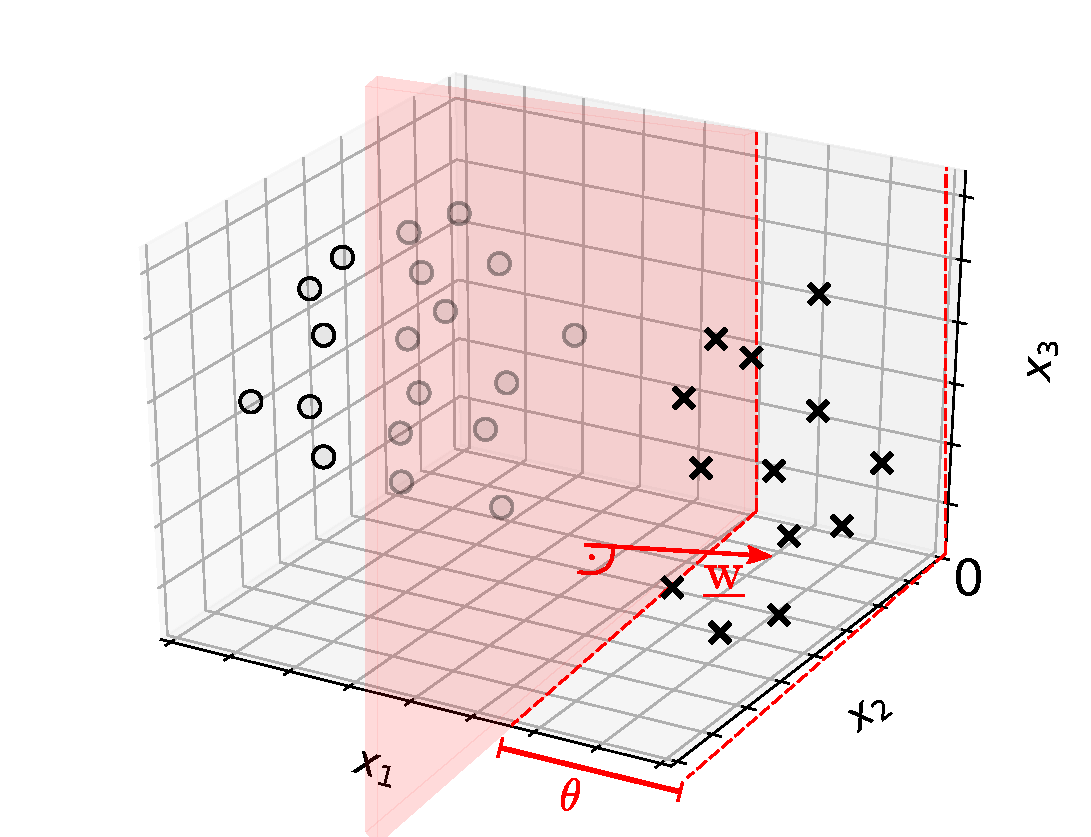
\includegraphics[height=6cm]{img/neuron_3d_grid_hyperplane.pdf}
        \caption{The plane divides the responses of the neuron. In the context of classification it is referred to as the decision boundary.}
        \label{fig:neuron_3d_grid_hyperplane}
    \end{figure}
    
\end{frame}
\begin{frame}{The input-output relationship}
    
    The input-output relationship is described by a linear filter with a static non-linearity $f(\cdot)$:

    \begin{equation}
        \label{eq:linearNeuron}
        y = f \Big(\; \underbrace{\sum_{j=1}^{N} {w}_{j} 
            {x}_j - \theta}_{=:h} \; \Big)
            = f \big(\;  \vec{w}^{\top}
            \vec{x}- \theta \; \big)
            = f(\,h\,)
    \end{equation}
    
	\[ \begin{array}{ll} 
		\vec{x}: & \text{input vector with components } \mathrm{x}_j \\
		y: & \text{scalar output of the neuron } \\
		\vec{w}: & \text{weight vector of the neuron with components }
			\mathrm{w}_{j}\\
		\theta: & \text{threshold of the neuron} \\
		h: & \text{total input of the neuron. } \\
		&\quad h \propto \frac{\vec w^\top \vec x}{\;||\vec w||_2} \text{ component of $\vec x$ in the direction of $\vec w$}\\
		f(\cdot): & \text{transfer function}
	\end{array} \]
    
\end{frame}

\begin{frame}

\question{What roles do the weights and bias play?}

\mode<article>{
\begin{itemize}
\item[-] $\vec w$ is effectively the normal vector of the hyperplane $\color{red}H = \{\vec x : \vec w^{\top} \vec x = \theta\}$. Therefore, the weights represent the orientation of the hyperplane (see. \figref{fig:neuron_3d_grid_hyperplane}).
\item[-] $\theta$ represents the shift of the hyperplane (see. \figref{fig:neuron_3d_grid_hyperplane}). It is the absolute position of the hyperplane fron the origin along $\vec w$. For any point $\widetilde{\vec x} \in H$ (i.e. points on the plane): 
$\frac{\vec w^\top \widetilde{\vec x}}{\,||\vec w||_2} = \frac{\theta}{\,||\vec w||_2}$
\end{itemize}
}

\mode<presentation>{
    \begin{figure}
        \centering
        \includegraphics<1>[width=0.5\textwidth]{img/neuron_3d_grid}
        \includegraphics<2>[height=0.5\textwidth]{img/neuron_3d_grid_hyperplane.pdf}
    \end{figure}
}
\end{frame}

\subsection{Linear vs. non-linear transfer functions}

\begin{frame}{Only}
\frametitle{Transfer functions}

\svspace{-4mm}

\question{What are the advantages of using a non-linear transfer function instead of a linear one?}

\svspace{-7mm}

\begin{figure}[ht]
     \centering
     \savebox{\imagebox}{
	 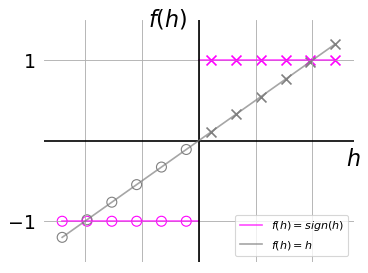
\includegraphics[width=0.3\textwidth]{img/neuron_1d_sign_and_linear}}%
     \begin{subfigure}[t]{0.35\textwidth}
         \centering
         \usebox{\imagebox}% Place largest image
         \caption{\footnotesize Linear vs. non-linear activation}
         \label{fig:linear_sign}
     \end{subfigure}
     \hspace{2mm}
     \begin{subfigure}[t]{0.35\textwidth}
         \centering
         \raisebox{\dimexpr.5\ht\imagebox-.5\height}{% Raise smaller image into place
         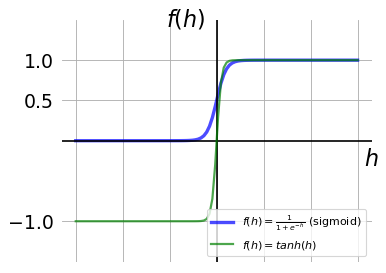
\includegraphics[width=0.9\textwidth]{img/neuron_1d_sigm_tanh}
         }
         \caption{\footnotesize logistic sigmoidal $\scriptstyle f(h)=\frac{1}{1+e^{-h}}$ vs. tanh}
         \label{fig:sigmoid_tanh}
     \end{subfigure}
     \mode<article>{
     \caption{Comparing linear with non-linear activation functions and differentiable alternatives to the sign function.}
     }
	 \label{fig:transfer_linear_nonlinear}
\end{figure}

\pause

\svspace{-7mm}

- Advantages:
\begin{enumerate}
\item<only@2> binary classification, either $f(h) \in \{0,1\}$ or $f(h) \in (-1,1)$
\item<only@3> interpret $f(h)$ as a probability. The logistic sigmoidal where $f(h) = \frac{1}{1+exp(-h)}$ yields values in the range of (0,1). \notesonly{The logistic sigmoidal can also be obtained by shifting and scaling the tanh function (see \sectionref{sec:tanh_to_sigmoid}.}
\item<only@4> a multilayer perceptron with only linear transfer functions can be reduced to a single layer.\notesonly{ The hidden layers become redundant }\only<4>{\footnote{Recent literature reveals interesting insights into what kind of representations arise during learning across the layers of linear networks. For more information see \citep{saxe2019mathematical}.}:\\

\notesonly{
     \begin{tabular}{c c c }
     		\raisebox{-9mm}{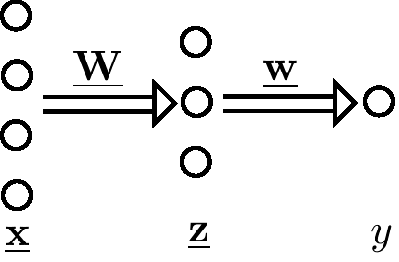
\includegraphics[height=2.25cm]{img/section1_fig16.pdf}}
     	& 
     		\begin{minipage}{10mm}
     			\vspace{10mm}
     		\end{minipage} 
     	& 
     		\parbox{4cm}{
		    \begin{eqnarray*}
		      y & = & \vec{w}^\top \vec{z}  
		      \quad = \quad \vec{w}^\top \vec{W} \, \vec{x} \\
		      & = & (\underbrace{\vec{W}^\top \vec{w}}_{=: \widehat{\vec{w}}})^\top \vec{x}
		      \quad = \quad \widehat{\vec{w}}^\top \vec{x}\\ 
		      & \corresponds & \text{connectionist neuron}
		    \end{eqnarray*}}
	\end{tabular}
}
}
\end{enumerate}


\end{frame}

\subsubsection{From logistic sigmoidal to tanh}
\label{sec:tanh_to_sigmoid}

%\begin{frame}

\mode<article>{
\question{How does the logistic sigmoidal function relate to the tanh function?}
}
%\mode<presentation>{

	%\only<1,2>{\placeimage{10}{3.5}{img/neuron_1d_sigm_tanh}{width=4.cm}}
%}

\mode<article>{

We observe in \figref{fig:sigmoid_tanh} that the logistic sigmoidal function (sigmoid) function is a shifted and scaled variant of the tanh function.

From this follows:

	\begin{align}
	f_{{\text{sigmoid}}}(h) 
    & = \frac{1}{1 + e^{-h}} \\
	& = \frac{e^{\frac{h}{2}}}{e^{\frac{h}{2}} + e^{-\frac{h}{2}}} \\
	& = \frac{1}{2} \Bigg(
		\underbrace{\frac{e^{\frac{h}{2}} - e^{-\frac{h}{2}}}{
			e^{\frac{h}{2}} + e^{-\frac{h}{2}}}}_{
				= \tanh \frac{h}{2}}
		+ \underbrace{\frac{
				e^{\frac{h}{2}} + e^{-\frac{h}{2}}
				%e^{h/2} + e^{-h/2}
				}
				{
				e^{\frac{h}{2}} + e^{-\frac{h}{2}}}}_{= 1}
		\Bigg) \\
	& = \frac{1}{2} \left( \tanh \frac{h}{2} + 1 \right)
	\end{align}
}
    
%\end{frame}

\subsection{Shortcut notation for weights and bias}

\begin{frame}{\subsecname}

\mode<article>{
The bias is effectively a connection between the neuron and an input that is always on. 
We can absorb the bias into the weight vector by prepending it to $\vec w$ and prepending $\vec x$ with an element $x_0 = 1$:
}

    \begin{figure}[h]
        \centering
        \only<1>{
        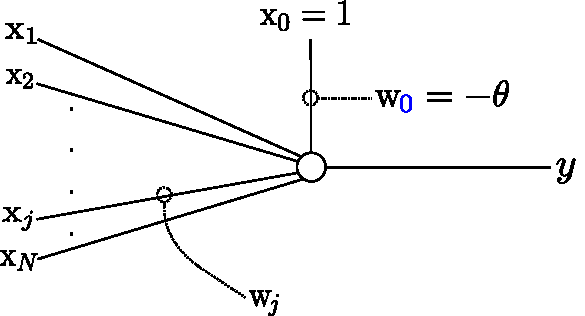
\includegraphics[height=3cm]{img/section1_fig6_highlight-bias}
        }
        \slidesonly{
        \only<2->{
        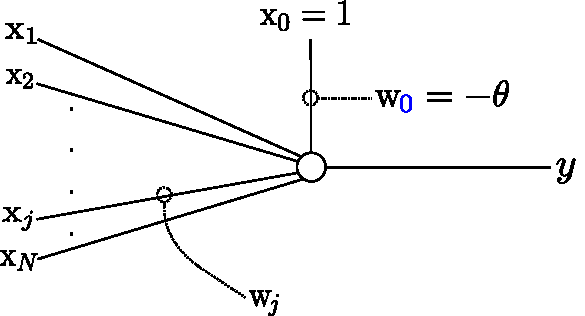
\includegraphics[height=2.2cm]{img/section1_fig6_highlight-bias}
        }
        }
         \caption{Absorb bias into weight vector.}
         \label{fig:weight_with_bias}
    \end{figure}
 
\only<1>{
\mode<article>{   
The response of the neuron depicted in \figref{fig:weight_with_bias} can be computed by:
}

\begin{equation}
	y = f\big( \sum_{{\color{blue}j=0}}^{N} \mathrm{w}_j \mathrm{x}_j \big)
		= f( \vec{w}^\top \vec{x} )
	\label{eq:weight_with_bias}
\end{equation}

\mode<article>{

Note that the sum in \eqref{eq:weight_with_bias} now iterates from ${\color{blue}j=0}$ instead of $j=1$ as was done in \eqref{eq:linearNeuron} in order to include the bias element.
}

}

\only<2>{

\svspace{-5mm}

	$\vec{w}$ will be used for $\rmat{ \mathrm{w}_1 \\ \vdots\;\,\\ \mathrm{w}_N}$ 
	as well as for $\rmat{ \mathrm{w}_{\color{blue}0} \\ \mathrm{w}_1 \\ \vdots\;\, \\ \mathrm{w}_N}$. \\
	
	\rule{2cm}{0pt}
	
	Accordingly,
	$\vec{x}$ will be used for $\rmat{ \mathrm{x}_1 \\ \vdots\;\,\\ \mathrm{x}_N}$ 
	as well as for $\rmat{ \mathrm{x}_{\color{blue}0} \\ \mathrm{x}_1 \\ \vdots\;\,\\ \mathrm{x}_N}$.
	
	\mode<article>{
	Whether the bias is absorbed or not should become apparent from the context or explicitly from the limits of the sum.
	}
}

\end{frame}
